\small УДК 517.938.5

\begin{center}{ \bf  Топология слоения Лиувилля биллиарда в области, ограниченной двумя софокусными эллипсами, в потенциальном поле}\\
{\it С.Е. Пустовойтов } \\
(Москва; {\it pustovoitovse1@mail.ru} )
\end{center}
\addcontentsline{toc}{section}{Пустовойтов С.Е.}


Биллиардом называется динамическая система на компактном подмножестве плоскости, описывающая  движение материальной точки внутри области  с абсолютно-упругим отражением на её границе. Рассмотрим биллиард в области, ограниченной двумя софокусными эллипсами, принадлежащими софокусному семейству, заданному формулой: $\frac{x^2}{a+\lambda}+\frac{y
^2}{b+\lambda}=1$, где $a>b>0$. Добавим в систему центральное поле сил. Следующие функции являются независимыми первыми интегралами данной системы: $H=\frac{k(x^2+y^2)}{2}+\frac{\dot{x}^2+\dot{y}^2}{2}$ и $F=\frac{\dot{x}^2}{a^2}+\frac{\dot{y}^2}{b^2}+\frac{(x\dot{y}-\dot{x}y)^2}{ab}-k(1-\frac{x^2}{a^2}-\frac{y^2}{b^2})$ [2]. Значит система вполне интегрируема.

\textbf{Теорема~1.} {\it Бифуркационная диаграмма для данной системы при $k>0$ изображена на рисунке №1. На рисунке №2 представленны грубые молекулы Фоменко-Цишанга [1], описывающие топологию изоэнергетических поверхностей $Q^3$, соответствующих уровням энергии 1, 2 и 3 интеграла Н.
}

\textbf{Теорема~2.} {\it Бифуркационная диаграмма для данной системы при $k<0$ изображена на рисунке №3. На рисунке №4 представленны грубые молекулы Фоменко-Цишанга [1], описывающие топологию изоэнергетических поверхностей $Q^3$, соответствующих уровням энергии 1, 2, 3, 4 и 5 интеграла Н.
}

%%%%  ОФОРМЛЕНИЕ СПИСКА ЛИТЕРАТУРЫ %%%
\smallskip \centerline{\bf Литература}\nopagebreak

1. Интегрируемые гамильтоновы системы. Геометрия, топология, классификация.// 	А.В. Болсинов, А.Т. Фоменко - том 1. Ижевск НИЦ	"Регулярная и хаотическая динамика", 1999

2. Некоторые интегрируемые обобщения задачи Якоби о геодезических на эллипсоиде/  Козлов В.В. // Прикладная математика и механика, том 59, вып.1, 1995

{\bf Пустовойтов Сергей Евгеньевич}, студент Московского государственного университета им.~М.В.~Ломоносова, г. Москва.

\begin{figure}[h]
  \center{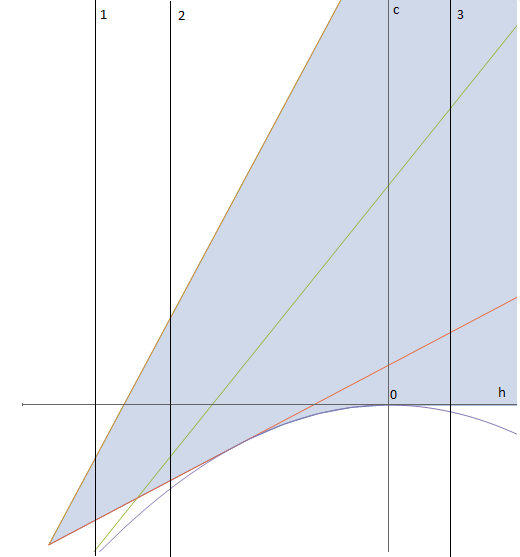
\includegraphics[width=35mm]{Pustovoytov_image3.png}}
  \caption{Бифуркационная диаграмма для случая $k>0$ (притяжение)} \label{void}
\end{figure}

\begin{figure}[h]
  \center{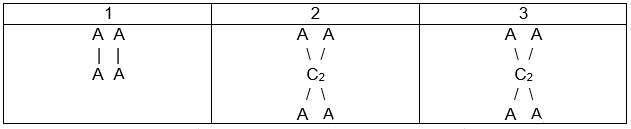
\includegraphics[width=45mm]{Pustovoytov_table1.png}}
  \caption{Грубые молекулы для случая $k>0$ (притяжение)}\label{void}
\end{figure}

\begin{figure}[h]
  \center{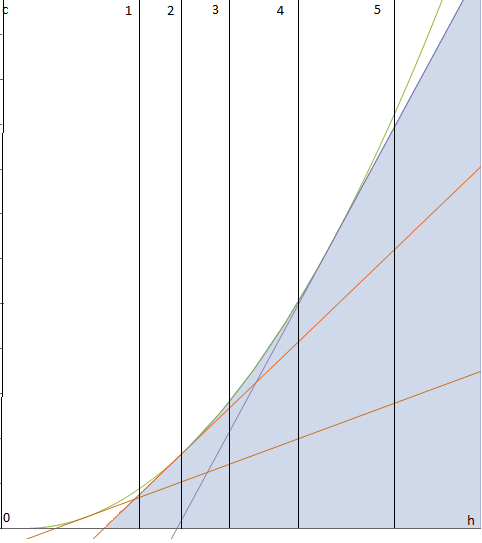
\includegraphics[width=35mm]{Pustovoytov_image2.png}}
  \caption{Бифуркационная диаграмма для случая $k<0$ (отталкивание)}\label{void}
\end{figure}

\begin{figure}[h]
  \center{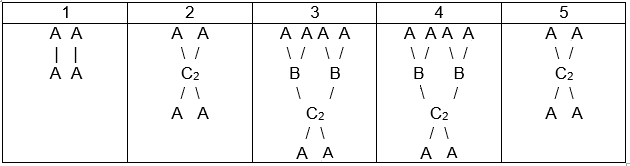
\includegraphics[width=45mm]{Pustovoytov_table2.png}}
  \caption{Грубые молекулы для случая $k<0$ (отталкивание)}\label{void}
\end{figure}

